\testCom
{%Номер задачи
	3.108
}
{%Условие
	условие
}
{%Дано
	дано
}
{%Найти
	$\omega_0$
}
{%Решение
	%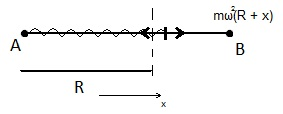
\includegraphics[height=30mm]{3_33.jpg}\\
	$\theta = \frac{\pi}{\lambda} = \frac{\omega'}{2 \beta} \sqrt{\frac{\omega_0^2}{4 \beta^2} - \frac{1}{4}}$\\
	$\arctg \frac{2 \beta \omega}{\omega_0^2 - \omega^2} = \varphi \Rightarrow 4 \beta^2 = \frac{(\omega^2 - \omega_0^2) \tg^2 \varphi}{\omega^2}$\\
	$\theta = \sqrt{\frac{\omega^2 \omega_0^2 \ctg^2 \varphi}{(\omega_0^2 - \omega^2)^2} - \frac{1}{4}} \quad \omega_0 : \der{x}{t}{2} + \omega_0^2 x = \der{x}{t}{2} \frac{\varkappa}{m} x = 0$\\
	$\omega_0 = \sqrt{\frac{\varkappa}{m}}$\\
}

